\usepackage{changepage}
\usepackage{float}
\usepackage{cite}
\usepackage{lipsum}
\usepackage{pstricks, caption}
\usepackage{url}
\usepackage[spanish, es-tabla]{babel}
\usepackage[shortlabels]{enumitem}
\usepackage{longtable,multirow,booktabs}
\usepackage{rotating}
\usepackage{caption}
\usepackage{multirow, array}
\usepackage{anyfontsize}
\usepackage{fix-cm}
\usepackage{calligra}
\usepackage{mathptmx}
\usepackage{caption}
\usepackage{fancyvrb}
%\usepackage{esvect}
\usepackage{xargs}
\usepackage{subfigure} 
\usepackage {titletoc}
\usepackage[T1]{fontenc}
%\usepackage[hyphens]{url}
\usepackage[breaklinks,colorlinks=true,linkcolor=blue,citecolor=red, urlcolor=blue]{hyperref}
\usepackage{flushend}


\documentclass[13,twocolumn,letterpaper]{article}
    \usepackage[spanish,english]{babel}
    \usepackage[utf8x]{inputenc}
    \usepackage[T1]{fontenc}
    \usepackage[a4paper,top=3cm,bottom=2cm,left=3cm,right=3cm,marginparwidth=1.75cm]{geometry}
    \usepackage{amsmath}
    \usepackage[colorinlistoftodos]{todonotes}
    \usepackage[colorlinks=true, allcolors=blue]{hyperref}
    \usepackage{float}
    
    
 \spanishdecimal{.}
\renewcommand{\figurename}{\textbf{Figura}}
\renewcommand{\tablename}{\textbf{Tabla}}
\renewcommand{\refname}{Bibliografía}
\renewcommand{\abstractname}{\large\textbf{Resumen}}
\renewcommand{\contentsname}{Contenido}
\renewcommand{\partname}{Parte}
\renewcommand{\appendixname}{Apéndice}
\renewcommand{\sin}{sen}	
\newenvironment{Figure}{\par\medskip\noindent\minipage{\linewidth}}{\endminipage\par\medskip}

    
    \title{
    		%\vspace{-1in} 	
    		\usefont{OT1}{bch}{b}{n}
    		\normalfont \normalsize \textsc{INSTITUTO POLITÉCNICO NACIONAL \\ 
    		ESCUELA SUPERIOR DE FISICA Y MATEMATICAS \\
    		ACADEMIA DE FÍSICA EXPERIMENTAL} \\ 
    		FÍSICA IV: LABORATORIO DE ÓPTICA. \\[10pt]
    		\huge Práctica X:\\
  Interferómetro de Michelson.\\
    }
    
    \usepackage{authblk}
    \author[0]{Alumno: Flores Rodriguez Jaziel David \\
    Boleta: 2014030429 \\
    Profesor: Dr. Janos Zsargo\\
    Grupo: 4FV2-B \\
            }
    \begin{document}
    
    \maketitle
   
    \selectlanguage{spanish}
    
    \section*{Resumen}
  Resumen: 
Durante esta práctica se presenta un experimento, con el fin de conocer qué es y cómo funciona el dispositivo denominado Interferómetro de Michelson. 
Para entender su funcionamiento, se presenta en la sección una breve introducción acerca del mismo. 
Posteriormente, se presenta el experimento llevado a cabo; uno muy sencillo de hecho, en el cual, usando un láser de luz verde y un interferómetro de Michelson, se pudo obtener la longitud de onda de este haz de luz.\\ 
 
 \begin{figure}[h]
	\centering
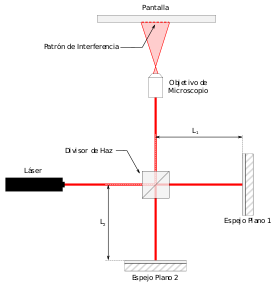
\includegraphics[width=\linewidth]{fig1.png}

	\label{fig:fig1}
\end{figure}


	\section*{Introducción}
El anterior diagrama muestra un interferómetro diseñado originalmente por Michelson, para probar la existencia del éter, medio hipotético en el cual se suponía que se propagaba la luz. \\

El haz luminoso emitido por el láser HeNe incide sobre el separador de haces, el cual refleja el 50\% de la onda incidente y transmite el otro 50\%. Uno de los haces se transmite hacia el espejo móvil M1 y el otro se refleja hacia el espejo fijo M2. Ambos espejos reflejan la luz hacia el separador de haces, de forma que los haces transmitido y reflejado por este último se recombinan sobre la pantalla de observación. \\

Como los dos haces que interfieren sobre la pantalla provienen de la misma fuente luminosa, la diferencia de fase se mantiene constante y depende sólo de la diferencia de camino óptico recorrido por cada uno. Por lo tanto, las franjas generadas por el interferómetro se pueden visualizar sobre la pantalla mediante la colocación de una lente convergente de corta distancia focal entre el láser y el separador de haces.  El sistema de franjas de interferencia producido es similar al que se muestra en la siguiente figura.\\

El camino óptico de uno de los haces se puede variar desplazando el espejo M1. Si dicho espejo se desplaza en $\frac{\lambda}{4}$ alejándose del separador de haces, el camino óptico de ese haz aumentará en $\frac{\lambda}{2}$. Las franjas de interferencia cambiarán de modo que el radio de los máximos aumentará y ocupará la posición de los mínimos iniciales. 
\\
Si el espejo M1 se desplaza en una distancia adicional de  $\frac{\lambda}{4}$, el nuevo sistema de franjas producido será indistinguible del original. 
 
\begin{figure}[h]
	\centering
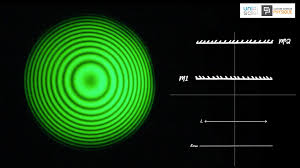
\includegraphics[width=\linewidth]{fig2.jpg}
\caption{Franjas de interferencia producidas por el interferómetro de Michelson. }
	\label{fig:fig2}
\end{figure}

Por lo tanto, desplazando lentamente el espejo en una distancia d y contando el número k de franjas que van pasando por un punto fijo de la pantalla, la longitud de onda de la luz se puede calcular como: 
\[\lambda = \frac{2d}{k}\]
		
\section*{Desarrollo experimental} 
Para la realización del experimento se hizo uso de un interferómetro de Michelson y un láser de luz verde; el sistema se montó como se muestra a continuación: 
 
\begin{figure}[h]
	\centering
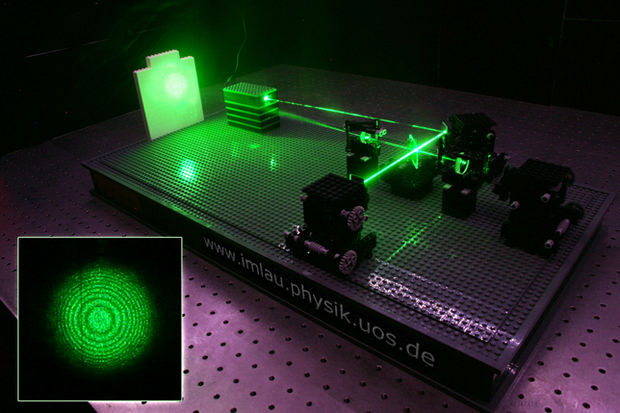
\includegraphics[width=\linewidth]{fig3.jpg}
\\
	\label{fig:fig3}
\end{figure}

El procedimiento fue el siguiente: \\

El interferómetro cuenta con un micrómetro que marca la distancia hacia el espejo móvil. \\

Cada vez que se movía el espejo móvil, el interferómetro emitía pulsos. \\

Se fue moviendo esta distancia hasta conseguir que se emitiesen k= 100 pulsos.\\ 

Hecho aquello, se tomó la distancia d que marcaba el micrómetro. \\

  
\begin{figure}[h]
	\centering
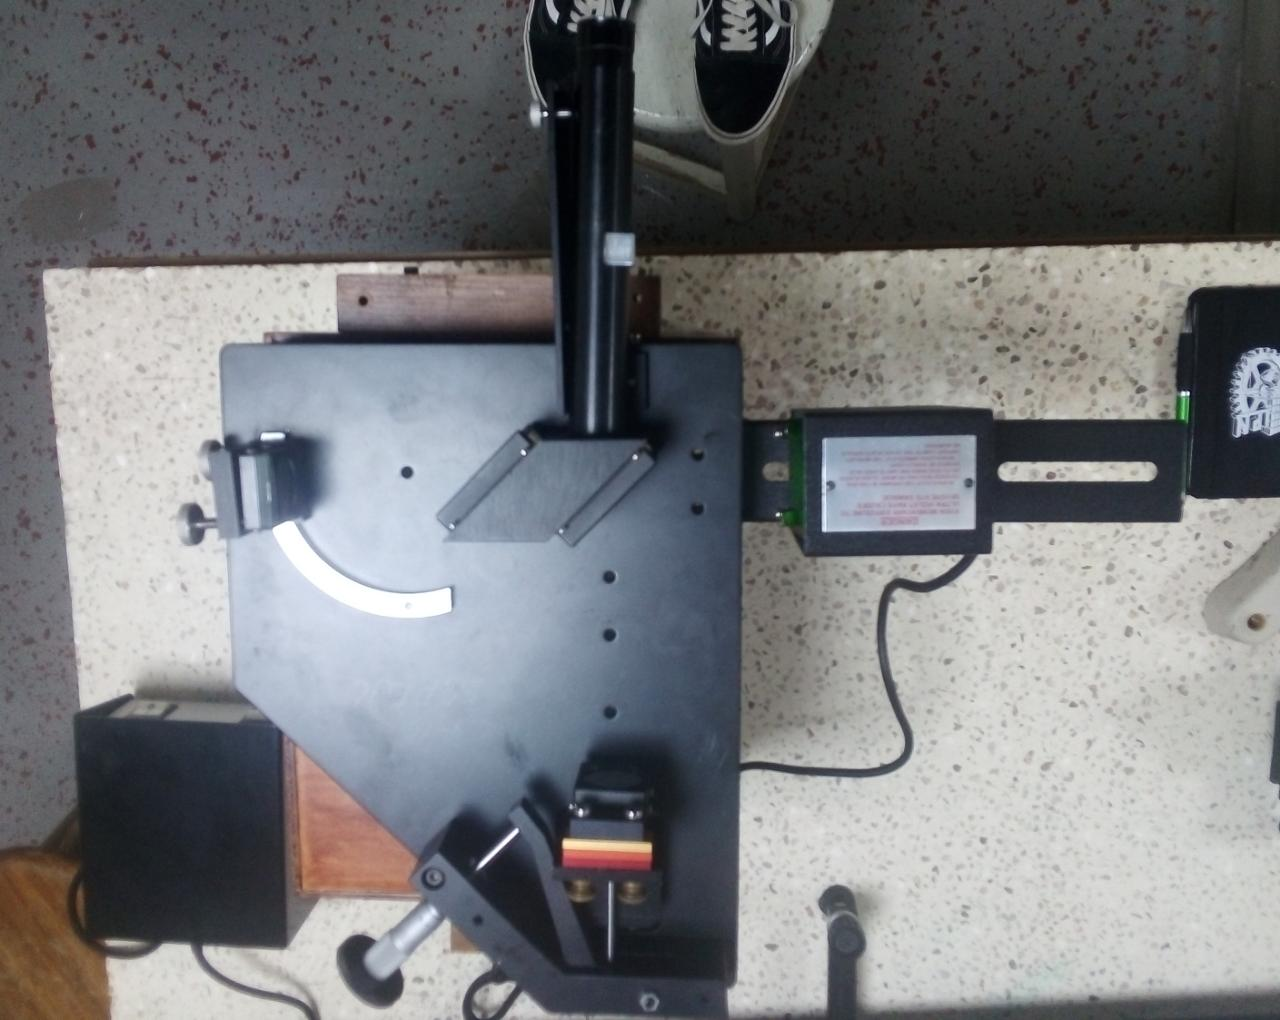
\includegraphics[width=\linewidth]{fig4.jpg}
	\label{fig:fig4}
\end{figure}

Cada integrante realizó una medición y los datos obtenidos se presentan en la sección de resultados.\\

\begin{figure}[h]
	\centering
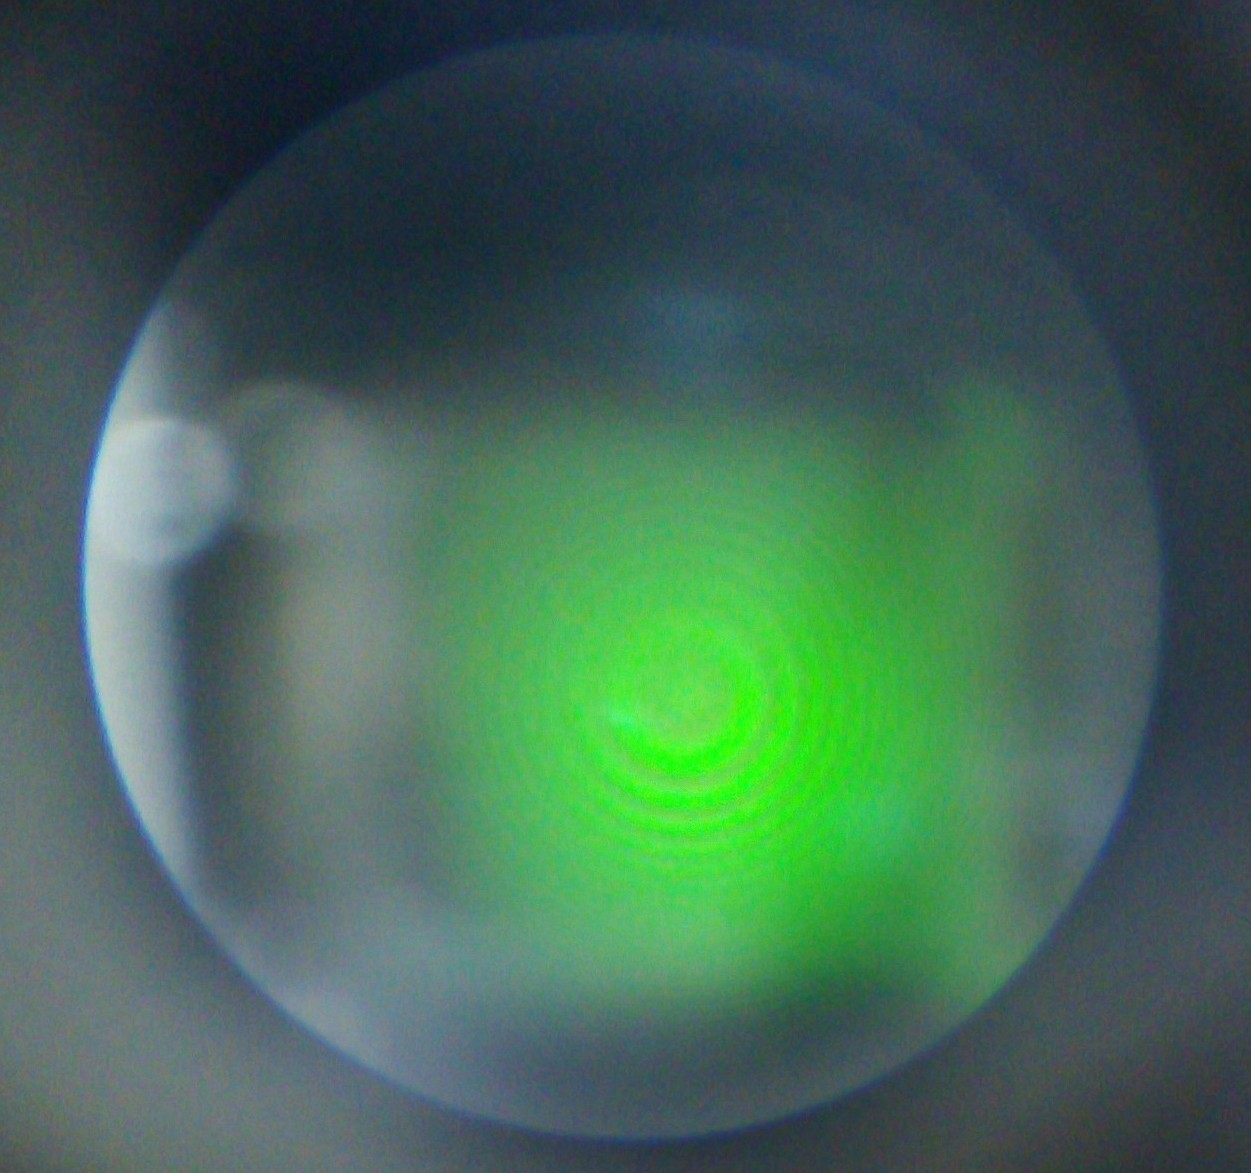
\includegraphics[width=0.8\linewidth]{fig5.jpg}
	\label{fig:fig5}
\end{figure}

\section*{Datos y resultados obtenidos}
A continuación, en la siguiente tabla se presentan los resultados obtenidos experimentalmente, así como los que se pudieron calcular conociendo estos:

\begin{table}[h]
    \centering
    \hline \hline\\
    Resultados del Experimento
    \hline \hline \\
    \begin{tabular}{|| c | c | c ||}
\hline \hline 
Número de Medición & \textbf{d}$(\mu m)$ & $\mathbf{\lambda}$ $(\mu m)$ \\ \hline
        1 & 17 & 0.34 \\ 
        2 & 20 & 0.4 \\ 
        3 & 35 & 0.7 \\ 
        4 & 19 & 0.38 \\ 
        5 & 19 & 0.38 \\ 
        6 & 19 & 0.38 \\
        7 & 16 & 0.32 \\\hline 
\textbf{Promedio} & 20.71 & 0.41 \\ \hline
    \end{tabular}
    \label{tab:my_label}
\end{table}

Se sabe además la longitud de onda de la luz verde, la cual es de ${\lambda}_{G}=$0.543 $(\mu m)$ (valor teórico). Así, calculando el error porcentual, se tiene: 

\[ e\% =  \frac{|0.543 − 0.41|}{0.543}\times 100 = 23.7 \% \]

Obteniendo un error porcentual por arriba del 20\%, el cual es  considerablemente alto,  ello muestra que el dato obtenido experimentalmente no es del todo bueno.

\section*{Conclusiones}
A pesar de que el interferómetro de Michelson es un dispositivo que permite calcular de manera rápida y sencilla la longitud de onda de un haz de luz, resulta inconveniente, ya que este depende de la percepción del observador al momento de que este decida cuando han sido 100 pulsaciones, ello de hecho puede ser motivo de que, como se pudo apreciar, este experimento no resultó ser del todo satisfactorio. 
Cabe mencionar además que, considerando lo anterior y el resultado obtenido, se podría obtener una mejor toma de datos si se pudiese hallar una manera más precisa de contar las pulsaciones. 
 


\nocite{Hecht}\nocite{Rossi}\nocite{Sears}\nocite{Born}\nocite{Tipler}\nocite{Feynman}\nocite{Res}
\bibliography{miBiblio.bib}
\bibliographystyle{plain}
\end{document}